%% -*- coding:utf-8 -*-

%%%%%%%%%%%%%%%%%%%%%%%%%%%%%%%%%%%%%%%%%%%%%%%%%%%%%%%%%
%%   $RCSfile: 5-merkmalstrukturen.tex,v $
%%  $Revision: 1.13 $
%%      $Date: 2010/11/16 08:40:32 $
%%     Author: Stefan Mueller (FU Berlin)
%%    Purpose: 
%%   Language: LaTeX
%%%%%%%%%%%%%%%%%%%%%%%%%%%%%%%%%%%%%%%%%%%%%%%%%%%%%%%%%




\chapter{Feature descriptions}
\label{chap-feature-descriptions}

In the previous chapter, we talked about sets of feature"=value pairs, which can be used to describe linguistic objects. In this chapter, we will introduce
feature descriptions which play a role in theories such as LFG, HPSG, Construction Grammar, versions of Categorial Grammar and TAG (and even some
formalizations of Minimalist theories \citep{Veenstra98a}). This chapter will therefore lay some of the groundwork for the chapters to follow.


Feature structures are complex entities which can model properties of a linguistic object. 
Linguists mostly work with feature descriptions which describe only parts of a given feature
structure. The difference between models and descriptions will be explained
in more detail in Section~\ref{sec-modelle-theorien}.

Alternative terms for feature structures are:
\begin{itemize}
\item feature"=value structure\is{feature"=value structure}
\item attribute"=value structure\is{attribute"=value structure}
\end{itemize}
Other terms for feature description are the following:
\begin{itemize}
\item \emph{attribute-value matrix} (AVM)
\item \emph{feature matrix}
\end{itemize}
In what follows, I will restrict the discussion to the absolutely necessary details in order to keep the formal part of the book as short as possible. I refer
the interested reader to \citet{Shieber86a}, \citet[Chapter~2]{ps}, \citet{Johnson88}, \citet{Carpenter92a},
\citet{King94a} and \citet{Richter2004a-u}. Shieber's book is an accessible introduction to Unification Grammars. The works by King and Richter, which introduce important
foundations for HPSG, would most probably not be accessible for those without a good grounding in mathematics. 
However, it is important to know that these works exist and that the corresponding linguistic theory is build on a solid foundation.

\section{Feature descriptions}

When\is{feature description|(} describing linguistic signs, we have to say something about their properties. For a noun, we can say that it has case, gender, number and person features.
For a word such as  \emph{Mannes} `man', we can say that these features have the values \emph{genitive}, \emph{masculine}, \emph{singular} and \emph{3}.
If we were to write these as a list of feature"=value pairs, we would arrive at the following feature description:
\eas
Feature-value pair for \emph{Mannes}:\\
\ms{
Case   & genitive\\
Gender   & masculine\\
Number & singular\\
Person  & 3\\
}
\zs
It is possible to describe a variety of different things using feature descriptions. For example, we can describe a person as in (\mex{1}):
\ea
\ms{
firstname    & max\\
lastname   & meier\\
date-of-birth & 10.10.1985\\
}
\z
People are related to other people -- a fact that can also be expressed in feature"=value pairs. For example, the fact that Max Meier has a father
called Peter Meier can be captured by expanding (\mex{0}) as follows: 
\ea
\ms{
firstname    & max\\
lastname   & meier\\
date-of-birth & 10.10.1985\\
father      & \ms{
             firstname & peter\\
             lastname  & meier\\
             date-of-birth   & 10.05.1960\\
             father     & \ldots\\
             mother     & \ldots\\
             }\\
mother     & \ldots\\
}
\z
The value of the \textsc{father} feature is another feature description containing the same features as (\mex{-1}).

In feature descriptions, a \emph{path}\is{path} is a sequence of features which immediately follow each other.
The \emph{value of a path} is the feature description at the end of the path. Therefore,
the value of \textsc{father$|$date-of-birth} is \emph{10.05.1960}.

One can think of many different features that could be included in representations such as (\mex{0}). One may wonder how
to integrate information about offspring into (\mex{0}).

An obvious solution would be to add features for \textsc{daughter} und \textsc{son}:
\ea
\ms{
firstname    & max\\
lastname  & meier\\
date-of-birth & 10.10.1985\\
father      & \ldots\\
mother     & \ldots\\
daughter    & \ldots\\   
}
\z
This solution is not satisfactory as it is not immediately clear how one could describe a person with several daughters.
Should one really introduce features such as \textsc{daughter-1} or \textsc{daughter-3}?
\ea
\ms{
firstname    & max\\
lastname  & meier\\
date-of-birth & 10.10.1985\\
father      & \ldots\\
mother     & \ldots\\
daughter-1    & \ldots\\   
daughter-2  & \ldots\\
daughter-3  & \ldots\\
}
\z
How many features do we want to assume? Where is the limit?
What would the value of \textsc{daughter"=32} be?

For this case, it makes much more sense to use a list\is{list}. Lists are indicated with angle brackets. Any number of elements can occur between
these brackets. A special case is when no element occurs between the brackets. A list with no
elements is also called \emph{empty list}. In the following example,
Max Meier has a daughter called Clara, who herself has no daughter.
\ea
\ms{
firstname    & max\\
lastname   & meier\\
date-of-birth & 10.10.1985\\
father      & \ldots\\
mother     & \ldots\\
daughter    & \liste{ \ms{
                     firstname    & clara\\
                     lastname   & meier\\
                     date-of-birth & 10.10.2004\\
                     father      & \ldots\\
                     mother     & \ldots\\
                     daughter   & \liste{ }\\   
} }\\   
}
\z
Now, we are left with the question of sons. Should we add another list for sons? Do we want to differentiate between sons and daughters?
It is certainly the case that the gender of the children is an important property, but these are
properties of the objects themselves, since every person has a gender. The description in (\mex{1}) therefore offers a more adequate representation.

\begin{figure}[tb]
\ea
\ms{
firstname    & max\\
lastname   & meier\\
date-of-birth & 10.10.1985\\
\textbf{gender} & \textbf{male}\\
father      & \ldots\\
mother     & \ldots\\
children    & \liste{ \ms{
                     firstname    & clara\\
                     lastname   & meier\\
                     date-of-birth & 10.10.2004\\
                     \textbf{gender} & \textbf{female}\\
                     father      & \ldots\\
                     mother     & \ldots\\
                     children     & \liste{ }\\   
} }\\   
}
\z
\vspace{-\baselineskip}
\end{figure}%
At this point, one could ask why the parents are not included in a list as well. In fact, we find similar questions also
in linguistic works: how is information best organized for the job at hand? One could argue for the
representation of descriptions of the parents under separate features, by pointing out that with
such a representation it is possible to make certain claims about a mother or father without having to necessarily
search for the respective descriptions in a list.

If the order of the elements is irrelevant, then we could use sets\is{set} rather than lists.
Sets are written inside curly brackets.\footnote{
The definition of a set requires many technicalities. 
In this book, sets would be used for the collection of semantic information only. This can be done equally
well using lists, which is why I do not introduce sets here and instead use lists.%
}

\section{Types}
\label{sec-formalismus-typen}

In\is{type|(} the previous section, we introduced feature descriptions consisting of feature"=value pairs and showed that it makes sense to allow for
complex values for features. In this section, feature descriptions will be augmented to include types. Feature descriptions which are assigned a type
are also called \emph{typed feature descriptions}. Types say something about which features can or must belong to a 
particular structure. The description previously discussed describes an object of the type \type{person}.
\ea
\ms[person]{
firstname    & max\\
lastname   & meier\\
date-of-birth & 10.10.1985\\
gender & male\\
father      & \ldots\\
mother     & \ldots\\
children     & \liste{ \ldots, \ldots{} }\\   
}
\z
Types are written in \textit{italics}. 

The specification of a type determines which properties a modelled object has. It is then only
possible for a theorie to say something about these properties.
Properties such as \textsc{operating voltage} are not relevant for objects of the type \textit{person}. If we know the type of a given object, then we
also know that this object must have certain properties even if we do not yet know their exact values. In this way, (\mex{1}) is still a description of
Max Meier even though it does not contain any information about Max' date of birth:
\ea
\ms[person]{
firstname   & max\\
lastname   & meier\\
gender & male\\
}
\z
We know, however, that Max Meier must have been born on some day since this is a description of the type \textit{person}.
The question \emph{What is Max' date of birth?} makes sense for a structure such as (\mex{0}) in a way that the question
\emph{Which operating voltage does Max have?} does not. If we know that an object is of the type \textit{person}, then we have
the following basic structure:
\ea
\ms[person]{
firstname    & firstname\\
lastname & lastname\\
date-of-birth & date\\
gender & gender\\
father      & person\\
mother    & person\\
children    & list of person\\   
}
\z
In (\mex{0}) and (\mex{-1}), the values of features such as \textsc{firstname} are in italics. These values are also types. They are different from
types such as \type{person}, however, as no features belong to them. These kinds of types are called \emph{atomic}\is{type!atomic}.

Types are organized into hierarchies\is{type hierarchy|(}.
It is possible to define the subtypes  \textit{woman} and \textit{man} for  \textit{person}. These would determine the gender of a given object.
(\mex{1}) shows the feature structure for the type \textit{woman}, which is analogous to that of \textit{man}.
\ea
\ms[female person]{
firstname    & firstname\\
lastname & lastname\\
date-of-birth & date\\
gender & female\\
father      & person\\
mother    & person\\
children    & list of person\\   
}
\z
At this point, we could ask ourselves if we really need the feature \textsc{gender}. The necessary information is already represented in the type \type{woman}.
The question if specific information is represented by special features or whether it is stored in a type without a corresponding individual feature will
surface again in the discussion of linguistic analyses.
Both alternatives differ mostly in the fact that the information which is modelled by types is not
immediately accessible for structure sharing, which is discussed in Section~\ref{sec-strukturteilung}.

Type hierarchies\label{Seite-Typhierarchie} play an important role in capturing linguistic generalizations, which is why type hierarchies and
the inheritance of constraints and information will be explained with reference to a further example in what follows. One can think of type hierarchies as an effective
way of organizing information. In an encyclopedia, the individual entries are linked in such a way that the entries for monkey and mouse will each contain a pointer
to mammal. The description found under mammal does therefore not have to be repeated for the subordinate concepts. In the same way, if one wishes to describe various
electric appliances, one can use the hierarchy in Figure~\vref{fig-electric-appliance}.
\begin{figure}
\centering
%% \begin{forest}
%% typehierarchy
%% [\type{electric appliance}
%%   [\type{printing device}
%%     [\type{printer}
%%       [\type{laser printer}]
%%       [\ldots]]
%%     [\subnode{copier}{\type{photocopier}}] ]
%%   [\subnode{scanning}{\type{scanning device}}
%%     [\type{scanner}
%%       [\type{negative scanner}]
%%       [\ldots] ] ]
%%   [\ldots]]
%% \draw (scanning.south)--(copier.north);
%% \end{forest}
\begin{tabular}{cccc}
\multicolumn{4}{c}{\mynode{ed}{\type{electric appliance}}}\\[6ex]
\mynode{p}{\type{printing device}} & & \mynode{sc}{\type{scanning device}} & \mynode{other}{\rule[-0.5ex]{0cm}{2.5ex}\ldots}\\[6ex]
\mynode{printer}{\type{printer}}   & \mynode{copy}{\type{photocopier}}  & \mynode{scanner}{\type{scanner}}\\[6ex]
\mynode{l-p}{\type{laser printer}}  & \mynode{other-p}{\rule[-0.5ex]{0cm}{2.5ex}\ldots}  & \mynode{negscan}{\type{negative scanner}} & \mynode{other-sc}{\rule[-0.5ex]{0cm}{2.5ex}\ldots}\\
\end{tabular}
\begin{tikzpicture}[overlay,remember picture,shorten <=2pt,shorten >=2pt] 
\draw(ed.south)--(p.north)
     (ed.south)--(sc.north)
     (ed.south)--(other.north)
     (p.south)--(copy.north)
     (p.south)--(printer.north)
     (printer.south)--(l-p.north)
     (printer.south)--(other-p.north)
     (sc.south)--(copy.north)
     (sc.south)--(scanner.north)
     (scanner.south)--(negscan.north)
     (scanner.south)--(other-sc.north);
\end{tikzpicture}
\caption{\label{fig-electric-appliance}Non"=linguistic example of multiple inheritance}
\end{figure}%
The most general type \type{electrical device} is the highest in Figure~\ref{fig-electric-appliance}. Electrical devices have certain properties, \eg, 
a power supply with a certain power consumption. All subtypes of  \type{electrical device} ``inherit'' this property. In this way, \type{printing device} and
\type{scanning device} also have a power supply with a specific power consumption. A
\type{printing device} can produce information and a \type{scanning device} can read in information. A \type{photocopier} can both produce information and read it. Photocopiers have both the properties of scanning and printing devices.
This is expressed by the connection between the two superordinate types and \type{photocopier} in
Figure~\ref{fig-electric-appliance}. If a type is at the same time the subtype of several superordinate types, then we
speak of \emph{multiple inheritance}\is{inheritance!multiple}. If devices can print, but not scan, they are of type \emph{printer}. This type can have further more
specific subtypes, which in turn may have particular properties, \eg, \type{laser printer}. New
features can be added to subtypes, but it is also possible to make values of inherited features more
specific. For example, the material that can be scanned with a \type{negative scanner} is far more
restricted than that of the supertype \type{scanner}, since negative scanners can only scan negatives.

The objects that are modeled always have a maximally specific type. In the example above, this means that we can have objects of the type \type{laser printer} and \type{negative scanner}
but not of the type \type{printing device}. This is due to the fact that \type{printing device} is not maximally specific since this type has two subtypes.

Type hierarchies with multiple inheritance are an important means for expressing linguistic generalizations \citep*{FPW85a,Flickinger87,Sag97a}. Types of words or phrases which
occur at the very top of these hierarchies correspond to constraints on linguistic objects, which are valid for linguistic objects in all languages. Subtypes of such general types
can be specific to certain languages or language classes.%
\is{type|)}\is{type hierarchy|)}

\section{Disjunction}

Disjunctions\is{disjunction|(} can be used if one wishes to express the fact that a particular object can have various different properties. If one were to organize a class reunion
twenty years after leaving school and could not recall the exact names of some former classmates, it would be possible to search the web for ``Julia (Warbanow or Barbanow)''. In
feature descriptions, this ``or'' is expressed by a `$\vee$'\is{$\vee$}.
\ea
\ms[person]{
firstname  & julia\\
lastname & warbanow $\vee$ barbanow\\
}
\z
Some internet search engines do not allow for searches with `or'. In these cases, one has to carry out two distinct search operations: one for ``Julia Warbanow'' and then another
for ``Julia Barbanow''. This corresponds to the two following disjunctively connected descriptions:
\ea
\ms[person]{
 firstname  & julia\\
 lastname & warbanow\\
} $\vee $
\ms[person]{
 firstname  & julia\\
 lastname & barbanow\\
}
\z
Since we have type hierarchies as a means of expression, we can sometimes do without disjunctive specification of values and instead state the supertype\is{type}:
for \type{printer} $\vee$  \type{photocopier}, one can simply write \type{printing device} if one assumes the type hierarchy in Figure~\vref{fig-electric-appliance}.%
\is{disjunction|)}

\section{Structure sharing}
\label{sec-strukturteilung}

Structure sharing\is{structure sharing|(} is an important part of the formalism. It serves to express the notion that certain parts of a structure are identical. A linguistic
example for the identity of values is agreement\is{agreement}. In sentences such as (\mex{1}), the number value of the noun phrase has to be identical to that of the verb:

\eal
\ex[]{
\gll Der Mann schläft.\\
	 the man sleeps\\
\glt `The man is sleeping.'
}
\ex[]{
\gll Die Männer schlafen.\\
	 the men sleep\\
\glt `The men are sleeping.'
}
\ex[*]{
\gll Der Mann schlafen.\\
	 the man sleep\\
\glt Intended: `The man are sleeping.'
}
\zl
The identity of values is indicated by boxes containing numbers. The boxes can also be viewed as
variables.

When describing objects we can make claims about equal values or claims about identical values.
A claim about the identity of values is stronger. Let us take the following feature description containing
information about the children that Max's father and mother have as an example:
\ea
\ms[person]{
firstname    & max\\
lastname   & meier\\
date-of-birth & 10.10.1985\\
father      & \ms[person]{
              firstname  & peter\\
              lastname & meier\\
              children   & \liste{ \ms[person]{
                                 firstname & klaus\\
                                 }, \ldots }\\
             }\\
mother    & \ms[person]{
              firstname  & anna\\
              lastname & meier\\
              children   & \liste{ \ms[person]{
                                 firstname & klaus\\
                                 }, \ldots }\\
             }\\
}
\z
Notice that under the paths \textsc{father$|$children} and \textsc{mother$|$children}, we find a list of a description of a person with the first name Klaus.
The question of whether the feature description is of one or two children of Peter and Anna cannot be answered. It is certainly possible that we are
dealing with two different children from previous partnerships who both happen to be called
Klaus.

By using structure sharing, it is possible to specify the identity of the two values:

\ea
\ms[person]{
firstname    & max\\
lastname   & meier\\
date-of-birth & 10.10.1985\\
father      & \ms[person]{
              firstname  & peter\\
              lastname & meier\\
              children   & \liste{ \ibox{1} \ms[person]{
                                 firstname & klaus\\
                                 }, \ldots }\\
             }\\
mother    & \ms[person]{
              firstname  & anna\\
              lastname & meier\\
              children & \liste{ \ibox{1}, \ldots }\\
             }\\
}
\z

In (\mex{0}), Klaus is a single child that belongs to both parents. Everything inside the brackets which immediately follow \iboxt{1} is equally present in both
positions. One can think of \iboxt{1} as a pointer or reference to a structure which has only been described once. One question still remains open: what about Max?
Max is also a child of his parents and should therefore also occur in a list of the children of his parents. There are two points in (\mex{0}) where there are three
dots. These ellipsis marks stand for information about the other children of Peter and Anna
Meier. Our world knowledge tells us that both of them must have the same child namely Max Meier himself. In the following section, we will see how this can be expressed in formal terms.%
\is{structure sharing|)}

\section{Cyclic structures}

We\is{cycle!in feature description|(} have introduced structure sharing in order to be able to express
the fact that Max's parents both have a son Klaus together. It would not be enough to list Max in
the child"=lists of his parents separately. We want to capture the fact that it is the same Max which
appears in each of these lists and furthermore, we have to ensure that the child being described is
identical to the entire object being described. Otherwise, the description would permit a situation where Max's
parents could have a second child also called Max.  The description given in
(\mex{1})\vpageref{bsp-avm-zyklen} can capture all facts correctly.
%\begin{figure}
\ea
\label{bsp-avm-zyklen}
\ibox{2} \ms[person]{
firstname    & max\\
lastname   & meier\\
date-of-birth & 10.10.1985\\
father      & \ms[person]{
              firstname  & peter\\
              lastname & meier\\
              children   & \liste{ \ibox{1} \ms[person]{
                                 firstname & klaus\\
                                 }, \ibox{2} }\\
             }\\
mother    & \ms[person]{
              firstname  & anna\\
              lastname & meier\\
              kinder   & \liste{ \ibox{1}, \ibox{2} }\\
             }\\
}
\z
%\vspace{-\baselineskip}\end{figure}%
Structures such as those described in (\mex{0}) are called cyclic because one ends up going in a circle if one follows a particular path: \eg, the path 
\textsc{father$|$""children$|$""\ldots$|$""father$|$""children$|$\ldots}\footnote{
	The dots here stand for the path to \iboxt{2} in the list which is the value of \textsc{children}. See Exercise~\ref{ua-liste}.%
}
can be potentially repeated an infinite number of times.
\is{cycle!in feature description|)}

\section{Unification}
\label{sec-unification}

\mbox{}\is{unification|(}%
Grammatical rules\todostefan{Read Ristad} are written exactly like lexical entries in HPSG and Construction Grammar and are done so with the help of feature descriptions.
For a word or a larger phrasal entity to be usable as daughter in a phrase licensed by some
grammatical rule, the word or phrase must have properties which are compatible with the description of the daughters in the grammatical rule. If
this kind of compatibility exists, then we can say that the respective items are \emph{unifiable}.\footnote{
	The term \emph{unification} should be used with care. It is only appropriate if certain assumptions with regard to the formal basis
	of linguistic theories are made. Informally, the term is often used in formalisms where unification is not technically defined. In HPSG, it mostly means that
	the constraints of two descriptions lead to a single description. What one wants to say here, intuitively, is that the objects described have to
	satisfy the constraints of both descriptions at the same time (\emph{constraint satisfaction}). Since the term \emph{unification} is so broadly-used,
	it will also be used in this section. The term will not play a role in the remaining discussions of theories with the exception of
	explicitly unification"=based approaches. In contrast, the concept of constraint satisfaction presented here is very important for the comprehension
	of the following chapters.%
}
If one unifies two descriptions, the result is a description which contains information from both descriptions but no additional information.

The way unification works can be demonstrated with feature descriptions describing people. One can imagine that Bettina Kant goes to the private detective
Max Müller and wants to find a specific person. Normally, those who go to a detective's office only come with a partial description of the person they
are looking for, \eg, the gender, hair color or date of birth. Perhaps even the registration number of the car belonging to the person is known.

It is then expected of the detective that he or she provides information fitting the description. If
we are looking for a blonde female named Meier (\mex{1}a), then we
do not want to get descriptions of a male red-head (\mex{1}b). The descriptions in (\mex{1}) are incompatible and cannot be unified:
\eal
\ex\label{ex-meier-female-blonde}
\ms[person]{
lastname   & meier\\
gender & female\\
haircolor  & blonde\\
}
\ex \ms[person]{
lastname   & meier\\
gender & male\\
haircolor & red\\
}
\zl
The description in (\mex{1}) would be a possible result for a search for a blonde, female individual called Meier:
\ea
\label{info-detective}
\ms[person]{
firstname    & katharina\\
lastname   & meier\\
gender & female\\
date-of-birth & 15.10.1965\\
haircolor  & blonde\\
}
\z
Katharina Meier could also have other properties unknown to the detective. The important thing is that the properties known to the detective match those
that the client is looking for. Furthermore, it is important that the detective uses reliable information and does not make up any information about the sought
object. The unification of the search in (\mex{-1}a) and the information accessible to the detective in (\mex{0}) is in fact (\mex{0}) and not (\mex{1}), for example:
\ea
\ms[person]{
firstname    & katharina\\
lastname   & meier\\
gender & female\\
date-of-birth & 15.10.1965\\
haircolor  & blond\\
children     & \liste{}\\
}
\z
(\mex{0}) contains information about children, which is neither contained in
(\ref{ex-meier-female-blonde}) nor in (\ref{info-detective}).
It could indeed be the case that Katharina Meier has no children, but there are perhaps several people
called Katharina Meier with the otherwise same properties. With this invented information, we might
exclude one or more possible candidates. 

It is possible that our detective Max Müller does not have any information about hair color in his
files. His files could contain the following information:
\ea
\ms[person]{
firstname   & katharina\\
lastname   & meier\\
gender & weiblich\\
date-of-birth & 15.10.1965\\
}
\z
These data are compatible with the search criteria. If we were to unify the descriptions in (\mex{-3}a) and (\mex{0}), we would get (\mex{-2}).
If we assume that the detective has done all his work, then Bettina Kant now knows that the person she is looking for has the properties of her
original search plus the newly discovered properties.
\is{unification|)}

\section{Phenomena, models and formal theories}
\label{sec-modelle-theorien}

In\is{model|(}\is{theory|(}\is{phenomenon|(}\is{feature structure|(} the previous sections, we introduced feature descriptions with types. These feature descriptions describe typed
feature structures, which are models of observable linguistic structures. In the definitions of types, one determines which properties of linguistic objects should be described.
The type hierarchy together with type definitions is also referred to as a \emph{signature}\is{signature}.
As a grammarian, one typically uses types in feature descriptions. These descriptions contain
constraints which must hold for linguistic objects. If no constraints are given, all values that are
compatible with the specification in the signature are possible values. For example, one can omit the case
description of a linguistic object such as \emph{Frau} `woman' since \emph{Frau} can -- as shown in (\mex{1}) -- appear in all four cases:

\eal\settowidth\jamwidth{(nominative)}
\ex 
\gll Die        Frau schläft. \\      
     the.\nom{} woman sleeps\\\jambox{(nominative)}
\ex 
\gll Wir gedenken der Frau. \\ 
     we commemorate the.\gen{} woman\\\jambox{(genitive)}
\ex 
\gll Er hilft der Frau.  \\    
     he helps the.\dat{} woman\\\jambox{(dative)}
\ex 
\gll Er liebt die Frau.   \\   
     he loves the.\acc{} woman\\\jambox{(accusative)}
\zl
In a given model, there are only fully specified representations, that is, the model contains four forms of \emph{Frau}, each with a different case.
For masculine nouns such as \emph{Mann} `man', one would have to say something about case in the description since the genitive"=singular form \emph{Mann-es}
differs from other singular forms, which can be seen by adding \emph{Mann} into the examples in (\mex{0}). (\mex{1}) shows the feature descriptions for
\emph{Frau} `woman' and \emph{Mann} `man':
\eal
\ex\label{avm-frau}
Frau `woman'\\*
\ms{
gender & fem\\
%kasus & Kasus\\
}
\ex\label{avm-mann}
Mann `man'\\
\ms{
gender & mas\\
case & nominative $\vee$ dative $\vee$ accusative~\\
}
\zl
Unlike (\mex{0}b), (\mex{0}a) does not contain a case feature since we do not need to say anything special about case in the description of \emph{Frau}.
Since all nominal objects require a case feature, it becomes clear that the structures for \emph{Frau} must actually also have a case feature.
The value of the case feature is of the type \type{case}. \type{case} is a general type which subsumes the subtypes \type{nominative}, \type{genitive},
\type{dative} and \type{accusative}. Concrete linguistic objects always have exactly one of these maximally specified types as their case value. The feature structures
belonging to (\mex{0}) are given in Figure~\ref{abb-avm-frau} and Figure~\ref{abb-avm-mann}.%\todostefan{dieabbildungfiguresref{abb-avm-frau}{abb-avm-mann}}

\begin{figure}
% scaling does not work with pstricks, so I first create the pdf and then scale, 24.10.2015
\oneline{%
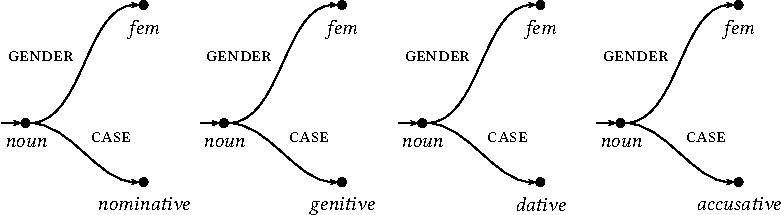
\includegraphics{Figures/frau-model-theoretic-cropped}
}
%%   \begin{pspicture}(-0.5,0.4)(2.8,4.1)
%% %\psgrid
%%      \psset{fillstyle=solid, fillcolor=black,radius=0.75mm}
%%      \pnode(-0.4,2){start1}
%%      \Cnode(0,2){noun1}
%%      \Cnode(2,4){fem1}
%%      \Cnode(2,1){nom1}
%% %
%%      \psset{fillstyle=none,nodesep=0pt,angleB=180,arrows=->} 
%% %
%%      \nccurve{start1}{noun1}
%%      \nccurve{noun1}{fem1}\naput{\textsc{gender}}
%%      \nccurve{noun1}{nom1}\naput{\textsc{case}}
%% %
%%      \nput{270}{noun1}{\type{noun}}
%%      \nput{270}{fem1}{\type{fem}}
%%      \nput{270}{nom1}{\type{nominative}}
%% \end{pspicture}
%% \begin{pspicture}(-0.5,0.4)(2.8,4.1)
%% %\psgrid
%% %
%%      \psset{fillstyle=solid, fillcolor=black,radius=0.75mm}
%%      \pnode(-0.4,2){start2}
%%      \Cnode(0,2){noun2}
%%      \Cnode(2,4){fem2}
%%      \Cnode(2,1){nom2}
%% %
%%      \psset{fillstyle=none,nodesep=0pt,angleB=180,arrows=->} 
%% %
%%      \nccurve{start2}{noun2}
%%      \nccurve{noun2}{fem2}\naput{\textsc{gender}}
%%      \nccurve{noun2}{nom2}\naput{~\textsc{case}}

%%      \nput{270}{noun2}{\type{noun}}
%%      \nput{270}{fem2}{\type{fem}}
%%      \nput{270}{nom2}{\type{genitive}}
%% \end{pspicture}
%% \begin{pspicture}(-0.5,0.4)(2.8,4.1)
%% %\psgrid
%%      \psset{fillstyle=solid, fillcolor=black,radius=0.75mm}
%%      \pnode(-0.4,2){start3}
%%      \Cnode(0,2){noun3}
%%      \Cnode(2,4){fem3}
%%      \Cnode(2,1){nom3}
%% %
%%      \psset{fillstyle=none,nodesep=0pt,angleB=180,arrows=->} 
%% %
%%      \nccurve{start3}{noun3}
%%      \nccurve{noun3}{fem3}\naput{\textsc{gender}}
%%      \nccurve{noun3}{nom3}\naput{\textsc{case}}
%% %
%%      \nput{270}{noun3}{\type{noun}}
%%      \nput{270}{fem3}{\type{fem}}
%%      \nput{270}{nom3}{\type{dative}}
%% \end{pspicture}
%% \begin{pspicture}(-0.5,0.4)(2.8,4.1)
%% %\psgrid
%%      \psset{fillstyle=solid, fillcolor=black,radius=0.75mm}
%%      \pnode(-0.4,2){start2}
%%      \Cnode(0,2){noun2}
%%      \Cnode(2,4){fem2}
%%      \Cnode(2,1){nom2}
%% %
%%      \psset{fillstyle=none,nodesep=0pt,angleB=180,arrows=->} 
%% %
%%      \nccurve{start2}{noun2}
%%      \nccurve{noun2}{fem2}\naput{\textsc{gender}}
%%      \nccurve{noun2}{nom2}\naput{\textsc{case}}
%% %
%%      \nput{270}{noun2}{\type{noun}}
%%      \nput{270}{fem2}{\type{fem}}
%%      \nput{270}{nom2}{\type{accusative}}
%% \end{pspicture}}
\caption{\label{abb-avm-frau}Feature structures for the description of \emph{Frau} `woman' in (\ref{avm-frau})}
\end{figure}%
%-----------------------------------------------------------------------------
\begin{figure}
%\oneline{%
\centerline{%
%% \begin{pspicture}(-0.5,0.4)(2.8,4.1)
%% %\psgrid
%% %
%% %
%%      \psset{fillstyle=solid, fillcolor=black,radius=0.75mm}
%%      \pnode(-0.4,2){start1}
%%      \Cnode(0,2){noun1}
%%      \Cnode(2,4){mas1}
%%      \Cnode(2,1){nom1}
%% %
%% %
%%      \psset{fillstyle=none,nodesep=0pt,angleB=180,arrows=->} 
%% %
%%      \nccurve{start1}{noun1}
%%      \nccurve{noun1}{mas1}\naput{\textsc{gender}}
%%      \nccurve{noun1}{nom1}\naput{\textsc{case}}
%% %
%%      \nput{270}{noun1}{\type{noun}}
%%      \nput{270}{mas1}{\type{mas}}
%%      \nput{270}{nom1}{\type{nominative}}
%% \end{pspicture}
%% \begin{pspicture}(-0.5,0.4)(2.8,4.1)
%% %\psgrid
%% %
%%      \psset{fillstyle=solid, fillcolor=black,radius=0.75mm}
%%      \pnode(-0.4,2){start2}
%%      \Cnode(0,2){noun2}
%%      \Cnode(2,4){mas2}
%%      \Cnode(2,1){nom2}
%% %
%% %
%%      \psset{fillstyle=none,nodesep=0pt,angleB=180,arrows=->} 
%% %
%%      \nccurve{start2}{noun2}
%%      \nccurve{noun2}{mas2}\naput{\textsc{gender}}
%%      \nccurve{noun2}{nom2}\naput{\textsc{case}}
%% %
%%      \nput{270}{noun2}{\type{noun}}
%%      \nput{270}{mas2}{\type{mas}}
%%      \nput{270}{nom2}{\type{dative}}
%% \end{pspicture}
%% \begin{pspicture}(-0.5,0.4)(2.8,4.1)
%% %\psgrid
%% %
%%      \psset{fillstyle=solid, fillcolor=black,radius=0.75mm}
%%      \pnode(-0.4,2){start2}
%%      \Cnode(0,2){noun2}
%%      \Cnode(2,4){mas2}
%%      \Cnode(2,1){nom2}
%% %
%% %
%%      \psset{fillstyle=none,nodesep=0pt,angleB=180,arrows=->} 
%% %
%%      \nccurve{start2}{noun2}
%%      \nccurve{noun2}{mas2}\naput{\textsc{gender}}
%%      \nccurve{noun2}{nom2}\naput{\textsc{case}}
%% %
%%      \nput{270}{noun2}{\type{noun}}
%%      \nput{270}{mas2}{\type{mas}}
%%      \nput{270}{nom2}{\type{accusative}}
%% \end{pspicture}
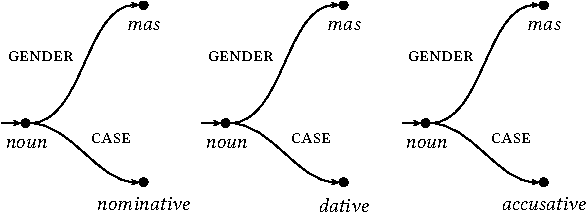
\includegraphics{Figures/mann-model-theoretic-crop}
}
\caption{\label{abb-avm-mann}Feature structures for the description of \emph{Mann} `man' in  (\ref{avm-mann})}
\end{figure}%
In these representations, each node has a certain type (\type{noun}, \type{fem}, \type{nominative},
\ldots) and the types in feature structures are always maximally specific, that is, they do not have
any further subtypes. There is always an entry node (\type{noun} in the example above) and the other
nodes are connected with arrows that are annotated with the feature labels (\textsc{gender}, \textsc{case}).

If we return to the example with people from the previous sections, we can capture the difference between a model and a description as follows:
if we have a model of people that includes first name, last name, date of birth, gender and hair color, then it follows that every object we model also has a birthday.
We can, however, decide to omit these details from our descriptions if they do not play a role for
stating constraints or formulating searches.

The connection between linguistic phenomena, the model and the formal theory is shown in Figure~\vref{abb-modell}.
\begin{figure}
\centerline{%
%{
%% \begin{pspicture}(0,0)(9.4,4.2)
%% %\psgrid
%% \rput[Bl](0,0){%
%% \begin{tabular}[b]{@{}ccc@{}}
%% phenomenon && model\\
%% \rnode{phen}{\fbox{\begin{tabular}{c}
%% linguistic\\
%% objects\\
%% \end{tabular}}}&&\rnode{modell}{\fbox{\begin{tabular}{c}
%% feature\\
%% structures\\
%% \end{tabular}}}\\[10ex]
%% &\rnode{theorie}{\fbox{\begin{tabular}{c}
%% feature\\
%% descriptions\\
%% \end{tabular}}}\\
%% &formal theory\\
%% \end{tabular}}
%% %\anodeconnect[l]{modell}[r]{phen}%
%% \ncline{->}{modell}{phen}\nbput{models}
%% %\ncdiag[angleA=180,angleB=45]{->}{modell}{theorie}
%% \psline{<-}(5.4,1.6)(6,2.4)
%% \rput[Bl](6,2){licensed by the theory} % früher Erfüllung, jetzt FR Änderung
%% \psline{->}(5,1.7)(5.6,2.4)
%% \rput[Bl](3.4,2.0){determines}
%% %\nccurve{<-}{modell}{theorie}\nbput{legt fest}
%% \ncline{->}{theorie}{phen}\naput{predicts}%
%% %\aanodeconnect[b]{modell}[tr]{theorie}%
%% %\anodeconnect[tl]{theorie}[b]{phen}%
%\end{pspicture}
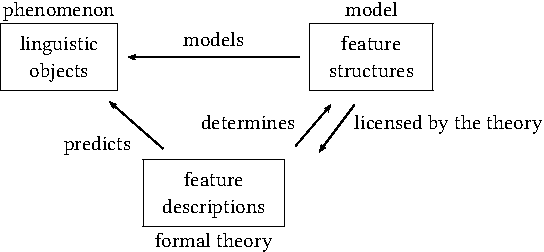
\includegraphics{Figures/model-theory-phenomenon-crop}
}
\caption{\label{abb-modell}Phenomenon, model and formal theory}
\end{figure}%
\nocite{Netter98a}%S. 26
%\NOTE{WS: zwischen Modell und Theorie sollten zwei Pfeile sein.}
% ###########
% zwei Pfeile: Beschreibung legt Modell fest , um Rekursion zu erfassen (beschreibt geht wohl auch, ist aber sloppy)
%
% Modell wird von der formalen Theorie lizenziert. 
%
% Phänomen + Modell -> PS: modelliert -> lassen wir so.
%
The model is designed to model linguistic phenomena. Furthermore, it must be licensed by our theory.
The theory determines the model and makes predictions with regard to possible phenomena.
\is{model|)}\is{theory|)}\is{Phenomenon|)}\is{feature description|)}\is{feature structure|)}


\section*{Comprehension questions}

\begin{enumerate}
\item What are the reasons for using types?
\item What is inheritance? What is special about multiple inheritance?
\item Are the following structures compatible, that is, can they be used to describe the same object? 
\ea
\onems{
firstname \type{max}\\
lastname \type{meier}\\
father    \ms[person]{
              firstname  & peter\\
              lastname & meier\\
             }\\
}\hspace{0.5cm}\onems{
firstname  \type{max}\\
lastname \type{meier}\\
father   \ms[person]{
              firstname  & peter\\
             lastname & müller\\
             }\\
}
\z
\ea
\onems{
firstname   \type{max}\\
lastname  \type{meier}\\
father     \ms[person]{
              firstname & peter\\
              lastname & meier\\
             }\\
}\hspace{0.5cm}\onems{
firstname   \type{max}\\
lastname  \type{meier}\\
mother      \ms[person]{
              firstname  & ursula\\
              lastname & müller\\
             }\\
}
\z

\end{enumerate}

\section*{Exercises}

\begin{enumerate}
\item Think about how one could describe musical instruments using feature descriptions.
\item Come up with a type hierarchy for the word classes (\type{det}, \type{comp}, \type{noun}, \type{verb},
      \type{adj}, \type{prep}). Think about the ways in which one can organize the type hierachy so that one
	  can express the generalizations that where captured by the binary features in Table~\ref{Tabelle-Merkmalszerlegung-Wortarten} on page~\pageref{Tabelle-Merkmalszerlegung-Wortarten}.
\item\label{ua-liste} In this chapter, we introduced lists. This may look like an extension of the formalism, but it is not as it is possible to
convert the list notation into a notation which only requires feature"=value pairs. Think about how one could do this.
\item (Additional exercise) The relation \emph{append}\is{relation!\emph{append}} will play a role in Chapter~\ref{Kapitel-HPSG}. This relation serves to
combine two lists to form a third.
Relational constraints such as \emph{append} do in fact constitute an expansion of the formalism. Using relational constraints, it is possible to relate any number
of feature values to other values, that is, one can write programs which compute a particular value depending on other values. 
This poses the question as to whether one needs such powerful descriptive tools in a linguistic theory and if we do allow them, what kind of complexity we afford them.
A theory which can do without relational constraints should be preferred over one that uses
relational constraints (see  \citew[Chapter~20]{MuellerLehrbuch1} for a comparison of theories).

For the concatenation of lists, there is a possible implementation in feature structures without
recourse to relational constraints. Find out how this can be done. Give your sources and document
how you went about finding the solution.

\end{enumerate}


\section*{Further reading}

This chapter was designed to give the reader an easy"=to"=follow introduction to typed feature structures. The mathematical properties of the structures, type hierarchies and the
combinatorial possibilities of such structures could not be discussed in detail here, but knowledge of
at least part of these properties is important for work in computational linguistics and in
developing one's own analyses. For more information, I refer the interested reader to the following publications: 
%
\citet{Shieber86a} is a short introduction to the theory of Unification Grammar. There is a relatively general overview followed by the discussion of important grammar types
such as DCG\is{Definite Clause Grammar (DCG)}, \lfg, \gpsg,
HPSG, PATR-II\is{PATR-II}.
%
\citet{Johnson88} describes the formalism of untyped feature structures in a mathematically precise way.
%
\citet{Carpenter92a} goes into the detail about the mathematical aspects of typed feature structures. The formalism developed by \citet{King99a-u} for HPSG"=grammars forms the basis
for the formalism by \citet{Richter2004a-u}, which currently counts as the standard formalism for HPSG.


%      <!-- Local IspellDict: en_US-w_accents -->
